\newpage
%=============================--A--=============================%
\renewcommand{\thefigure}{E\arabic{figure}}
\renewcommand{\thetable}{E\arabic{table}}
\setcounter{figure}{0}
\section{Exposição de dados}
\subsection{E.1 Método de obtenção de dados}

A extração de dados foi realizada primariamente com recurso a dois \textit{scripts} desenvolvidos em \textit{Python}:
\vskip -0.25em
\begin{lstlisting}[caption=\textit{Source code}: \color{white}{\underline{\textit{Script} responsável pela comparação de ficheiros} (bit\_error.py)}, frame=tlrb]{saucecode1}
#!/bin/python3
def bit_error(B):
    file_s = "sent.dat";
    file_r = "received.dat";
    
    if B:
        OFFSET = 49;
    else:
        OFFSET = 49*2;

    SIZE = 27*8;
    bit_errors = 0;
    sent = ""; received = "";
#-----
    read_s = open(file_s,'rb').read(); 
    read_r = open(file_r,'rb').read(); 

    for s in read_s:
        sent += '{0:08b}'.format(s);
    for r in read_r:
        received += '{0:08b}'.format(r);

    for i in range(0, SIZE):
        #print((sent[i], received[i+OFFSET]))
        if(sent[i] != received[i+OFFSET]):
            bit_errors += 1;

    print("SENT: \n" + sent[:SIZE] + "\n")
    print("RECEIVED: \n" + received[OFFSET:OFFSET+SIZE])

    print("Bit errors: " + str(bit_errors));
    return bit_errors

\end{lstlisting}
\vskip -0.75em
\begin{lstlisting}[caption=\textit{Source code}: \color{white}{\underline{\textit{Script} responsável pela automatização da comparação de ficheiros} (sim.py)}, frame=tlrb]{saucecode2}
#!/bin/python3
import signal
from bit_error import bit_error 

B=True;
BW = 0.0; N = 0.0;

if B:
    from mdBPSK_copy import mdBPSK as top_block_cls
else:
    from mdQPSK_copy import mdQPSK as top_block_cls

#-----
def sim():
    N0 = [x/2 for x in range(9)];
    loop_BW = [round(6/100 * x/10, 3) for x in range(1,43)];
    #---
    f = open("data.csv", "w"); f.write("N,BW,bit_errors\n")
    #--- .csv
    for N in N0:
        for BW in loop_BW:
            tb = top_block_cls(BW,N); #simulação
            tb.start();
            #tb.show();
            tb.wait();
            b = bit_error(B);
            f.write(str(N) + "," + str(BW) + "," + str(b) + "\n");

    tb.show();
    #---
    f.close();
    #---
    def sig_handler(sig=None, frame=None):
        tb.stop();
        tb.wait();
    #---
    signal.signal(signal.SIGINT, sig_handler);
    signal.signal(signal.SIGTERM, sig_handler);
\end{lstlisting}

As alterações necessárias foram aplicadas aos ficheiros \textit{Python} criados de forma automática pelo \textit{software} \textit{GNU Radio} de modo a que se tornassem suscetíveis à automatização requerida para a análise de dados significantes subsequente.

\label{sec:analise}
%=============================--A--=============================%
%\definecolor{green}{rgb}{0.1,0.1,0.1}
\subsection{E.2 Análise do sistema BPSK}
\label{sec:analiseBPSK}
\vskip -0.5em
\begin{table}[H]
\caption{Taxa de erro de \textit{bit} em função da \textit{Loop Bandwidth}, para cada \textit{noise voltage}.}
\vskip -0.5em
\label{tab:bpsk}
\hspace*{-0.75cm}\begin{tabular}{|c|c|c|c|c|c|c|c|c|c|}
\hline
Loop BW/Noise & 0.0 & 0.5 & 1.0 & 1.5 & 2.0 & 2.5 & 3.0 & 3.5 & 4.0 \\
\hline\hline
0.006 &\cellcolor{green!25}0.0\% & 1.4\% & 9.7\% & 19.0\% & 25.5\% & 30.6\% & 34.7\% & 38.0\% & 39.4\% \\
\hline
0.012 &\cellcolor{green!25}0.0\% & 1.4\% & 9.7\% & 19.0\% & 25.0\% & 29.6\% & 34.3\% & 35.6\% & 38.0\% \\
\hline
0.018 &\cellcolor{green!25}0.0\% & 1.4\% & 9.7\% & 19.4\% & 25.0\% & 28.7\% & 33.3\% & 36.6\% & \cellcolor{green!25}33.8\% \\
\hline
0.024 &\cellcolor{green!25}0.0\% & 1.4\% & 9.7\% & 19.4\% & \cellcolor{green!25}24.5\% & 29.6\% & 34.7\% & 39.4\% & 34.3\% \\
\hline
0.03 &\cellcolor{green!25}0.0\% & 1.4\% & 9.7\% & 19.0\% & \cellcolor{green!25}24.5\% & 29.6\% & 34.7\% & 34.3\% & 37.5\% \\
\hline
0.036 &\cellcolor{green!25}0.0\% & 1.4\% & 9.7\% & 19.0\% & 25.0\% & 28.7\% & \cellcolor{green!25}31.0\% & \cellcolor{green!25}33.3\% & 38.9\% \\
\hline
0.042 &\cellcolor{green!25}0.0\% & 1.4\% & 9.7\% & 18.5\% & 25.0\% & 37.0\% & 32.4\% & 34.3\% & 39.8\% \\
\hline
0.048 &\cellcolor{green!25}0.0\% & 1.4\% & 9.3\% & 18.5\% & \cellcolor{green!25}24.5\% & \cellcolor{green!25}28.2\% & \cellcolor{green!25}31.0\% & 36.1\% & 44.9\% \\
\hline
0.054 &\cellcolor{green!25}0.0\% &\cellcolor{green!25}0.9\% & 9.7\% & 18.5\% & 35.2\% & 31.5\% & \cellcolor{green!25}31.0\% & 38.0\% & 39.4\% \\
\hline
0.06 &\cellcolor{green!25}0.0\% &\cellcolor{green!25}0.9\% & 9.3\% & 20.8\% & 25.0\% & 28.7\% & 34.7\% & 50.0\% & 43.1\% \\
\hline
0.066 &\cellcolor{green!25}0.0\% &\cellcolor{green!25}0.9\% & 9.3\% & 20.4\% & 25.0\% & \cellcolor{green!25}28.2\% & 34.7\% & 40.3\% & 41.2\% \\
\hline
0.072 &\cellcolor{green!25}0.0\% &\cellcolor{green!25}0.9\% & 8.8\% & 19.9\% & 25.9\% & 27.3\% & 33.3\% & 56.0\% & 55.1\% \\
\hline
0.078 &\cellcolor{green!25}0.0\% &\cellcolor{green!25}0.9\% & 10.6\% & 19.0\% & 27.3\% & 29.2\% & 40.7\% & 40.3\% & 44.4\% \\
\hline
0.084 &\cellcolor{green!25}0.0\% &\cellcolor{green!25}0.9\% & 12.0\% & 19.4\% & 26.9\% & 29.6\% & 37.5\% & 35.6\% & 42.6\% \\
\hline
0.09 &\cellcolor{green!25}0.0\% &\cellcolor{green!25}0.9\% & 11.6\% & \cellcolor{green!25}16.7\% & 27.8\% & 38.4\% & 41.2\% & 56.9\% & 51.4\% \\
\hline
0.096 &\cellcolor{green!25}0.0\% &\cellcolor{green!25}0.9\% & 11.6\% & 17.1\% & 25.9\% & 38.4\% & 48.1\% & 32.4\% & 49.5\% \\
\hline
0.102 &\cellcolor{green!25}0.0\% &\cellcolor{green!25}0.9\% & 10.2\% & 19.9\% & 25.5\% & 41.7\% & 44.4\% & 42.1\% & 50.5\% \\
\hline
0.108 &\cellcolor{green!25}0.0\% &\cellcolor{green!25}0.9\% & 9.7\% & 20.4\% & 25.5\% & 38.4\% & 49.1\% & 46.3\% & 54.2\% \\
\hline
0.114 &\cellcolor{green!25}0.0\% &\cellcolor{green!25}0.9\% & 8.8\% & 23.1\% & 30.1\% & 37.0\% & 47.7\% & 42.1\% & 50.0\% \\
\hline
0.12 &\cellcolor{green!25}0.0\% &\cellcolor{green!25}0.9\% & \cellcolor{green!25}7.4\% & 18.5\% & 39.8\% & 44.4\% & 51.9\% & 48.1\% & 49.5\% \\
\hline
0.126 &\cellcolor{green!25}0.0\% &\cellcolor{green!25}0.9\% & 7.9\% & 21.3\% & 40.7\% & 33.3\% & 48.6\% & 47.7\% & 46.3\% \\
\hline
0.132 &\cellcolor{green!25}0.0\% &\cellcolor{green!25}0.9\% & 9.3\% & 19.9\% & 44.0\% & 33.3\% & 47.2\% & 53.7\% & 48.6\% \\
\hline
0.138 &\cellcolor{green!25}0.0\% &\cellcolor{green!25}0.9\% & 10.6\% & 21.8\% & 37.5\% & 37.0\% & 48.1\% & 47.7\% & 50.0\% \\
\hline
0.144 &\cellcolor{green!25}0.0\% &\cellcolor{green!25}0.9\% & 8.3\% & \cellcolor{green!25}16.7\% & 37.5\% & 44.9\% & 50.5\% & 44.0\% & 53.7\% \\
\hline
0.15 &\cellcolor{green!25}0.0\% &\cellcolor{green!25}0.9\% & 8.3\% & 19.0\% & 38.0\% & 39.4\% & 43.1\% & 44.9\% & 53.2\% \\
\hline
0.156 &\cellcolor{green!25}0.0\% &\cellcolor{green!25}0.9\% & 10.6\% & 17.1\% & 28.2\% & 36.1\% & 47.7\% & 53.2\% & 50.5\% \\
\hline
0.162 &\cellcolor{green!25}0.0\% &\cellcolor{green!25}0.9\% & 9.7\% & 19.0\% & 44.0\% & 35.2\% & 44.4\% & 44.4\% & 53.7\% \\
\hline
0.168 &\cellcolor{green!25}0.0\% &\cellcolor{green!25}0.9\% & 9.7\% & 21.8\% & 31.9\% & 48.1\% & 41.7\% & 52.3\% & 51.9\% \\
\hline
0.174 &\cellcolor{green!25}0.0\% &\cellcolor{green!25}0.9\% & 9.3\% & 27.8\% & 39.8\% & 43.1\% & 53.7\% & 50.5\% & 44.4\% \\
\hline
0.18 &\cellcolor{green!25}0.0\% &\cellcolor{green!25}0.9\% & 8.8\% & 31.0\% & 48.6\% & 50.5\% & 45.4\% & 53.2\% & 47.2\% \\
\hline
0.186 &\cellcolor{green!25}0.0\% &\cellcolor{green!25}0.9\% & 9.3\% & 30.6\% & 42.1\% & 44.4\% & 52.3\% & 57.9\% & 46.8\% \\
\hline
0.192 &\cellcolor{green!25}0.0\% &\cellcolor{green!25}0.9\% & 11.6\% & 21.8\% & 48.1\% & 42.6\% & 51.9\% & 52.3\% & 49.5\% \\
\hline
0.198 &\cellcolor{green!25}0.0\% & 1.4\% & \cellcolor{green!25}7.4\% & 21.3\% & 45.8\% & 52.8\% & 45.4\% & 46.8\% & 47.2\% \\
\hline
0.204 &\cellcolor{green!25}0.0\% & 1.4\% & 8.3\% & 39.8\% & 44.4\% & 57.9\% & 51.4\% & 49.1\% & 51.9\% \\
\hline
0.21 &\cellcolor{green!25}0.0\% &\cellcolor{green!25}0.9\% & 16.2\% & 42.6\% & 34.3\% & 30.6\% & 50.5\% & 45.8\% & 50.5\% \\
\hline
0.216 &\cellcolor{green!25}0.0\% & 1.9\% & 23.6\% & 40.7\% & 43.5\% & 40.3\% & 43.5\% & 45.8\% & 50.5\% \\
\hline
0.222 &\cellcolor{green!25}0.0\% & 1.4\% & 13.9\% & 53.2\% & 44.0\% & 53.2\% & 51.9\% & 44.4\% & 50.9\% \\
\hline
0.228 &\cellcolor{green!25}0.0\% & 1.9\% & 12.5\% & 19.9\% & 36.6\% & 48.6\% & 47.2\% & 48.1\% & 49.5\% \\
\hline
0.234 &\cellcolor{green!25}0.0\% & 8.3\% & 10.6\% & 31.9\% & 25.9\% & 47.2\% & 48.6\% & 45.8\% & 54.6\% \\
\hline
0.24 &\cellcolor{green!25}0.0\% &\cellcolor{green!25}0.9\% & 11.1\% & 38.9\% & 36.6\% & 44.9\% & 44.4\% & 50.5\% & 51.9\% \\
\hline
0.246 &\cellcolor{green!25}0.0\% & 1.4\% & 12.5\% & 38.4\% & 46.8\% & 49.1\% & 52.8\% & 50.5\% & 42.1\% \\
\hline
0.252 &\cellcolor{green!25}0.0\% & 1.4\% & 28.7\% & 21.8\% & 49.5\% & 44.9\% & 45.4\% & 43.5\% & 52.3\%\\
\hline
\end{tabular}
\end{table}

%---
\begin{figure}[H]
    \centering
    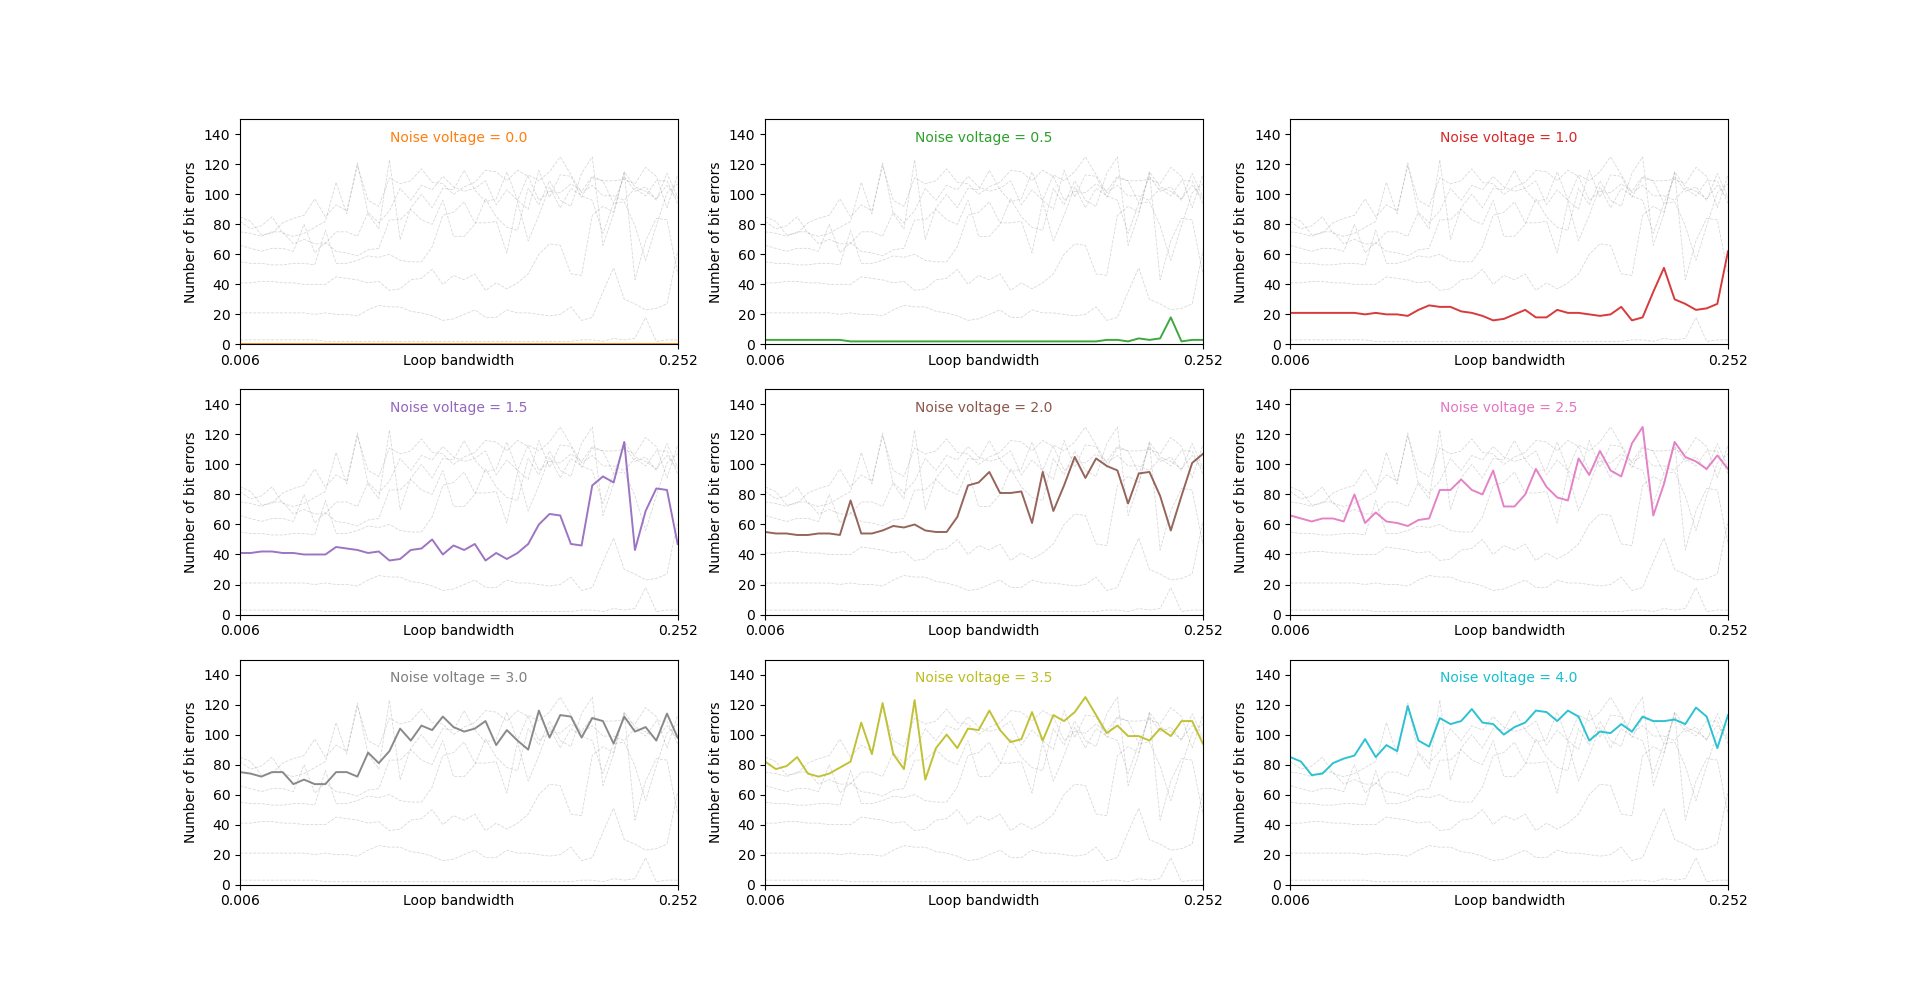
\includegraphics[width=1\linewidth]{img/analise/BPSK_9.png}
    \caption{Evolução do número de erros de \textit{bit} para cada \textit{noise voltage}, em função da \textit{Loop Bandwidth}.}
    \label{fig:bpsk9}
\end{figure}

\noindent\fcolorbox{black}{white}{%
        \minipage[t]{\dimexpr\linewidth-2\fboxsep-2\fboxrule\relax}
            \textbf{Observação 1} $\rightarrow$ Verifica-se, como esperado, um número de erros cada vez mais prevalente e mais oscilante para valores de \textit{Loop Bandwidth} cada vez mais distantes de zero (distanciamento da gama ótima de valores\cite{symbolsync-gnuradio} discutida anteriormente na \hyperref[subsubsec:symbol-sync]{secção 3.1}). É também de salientar a proporcionalidade observada (e expectável) do número de erros de \textit{bit} com o patamar de ruído (aumento da dificuldade em detetar o pulso no seio do ruído $\implies$ maior taxa de erro de \textit{bit}).
        \endminipage}

\vskip 1em
\noindent\fcolorbox{black}{white}{%
        \minipage[t]{\dimexpr\linewidth-2\fboxsep-2\fboxrule\relax}
            \textbf{Observação 2} $\rightarrow$ Para cada gráfico é aparente uma zona de maior estabilidade (número de erros bastante próximos) que tende a contrair e a mutar para uma extensão cada vez mais instável, com o aumento da \textit{noise voltage}. 
        \endminipage}

\vskip 1em
\noindent\fcolorbox{black}{white}{%
        \minipage[t]{\dimexpr\linewidth-2\fboxsep-2\fboxrule\relax}
            \textbf{Nota} $\rightarrow$ Encontram-se a \textcolor{green}{verde} na tabela os valores da \textit{Loop Bandwidth} que minimizam a taxa de erro de \textit{bit} para cada patamar de ruído no sistema BPSK projetado. A segunda observação é corroborada por estes valores \textit{highlighted}, dado que o valor ótimo de \textit{Loop Bandwidth} aparenta tender para valores nominalmente mais próximos de zero com o aumento da \textit{noise voltage}. 
        \endminipage}
%=============================--A--=============================%
\subsection{E.3 Análise do sistema QPSK}
\label{sec:analiseQPSK}
\vskip -0.5em
\begin{table}[H]
\caption{Taxa de erro de \textit{bit} em função da \textit{Loop Bandwidth}, para cada \textit{noise voltage}.}
\vskip -0.5em
\label{tab:qpsk}
\hspace*{-0.75cm}\begin{tabular}{|c|c|c|c|c|c|c|c|c|c|}
\hline
Loop BW/Noise & 0.0 & 0.5 & 1.0 & 1.5 & 2.0 & 2.5 & 3.0 & 3.5 & 4.0 \\
\hline\hline
0.006 & \cellcolor{green!25}0.0\% & 1.9\% & 11.1\% & 19.0\% & 28.2\% & 31.5\% & 34.3\% & 36.6\% & 38.0\% \\
\hline
0.012 & \cellcolor{green!25}0.0\% & 1.4\% & 11.1\% & 19.0\% & 27.8\% & 31.0\% & 33.8\% & 35.6\% & 37.5\% \\
\hline
0.018 & \cellcolor{green!25}0.0\% & 1.4\% & 10.6\% & 18.5\% & 26.4\% & 30.6\% & 33.3\% & 36.6\% & \cellcolor{green!25}32.9\% \\
\hline
0.024 & \cellcolor{green!25}0.0\% & 1.4\% & 10.6\% & 18.1\% & 26.9\% & 29.6\% & 33.3\% & \cellcolor{green!25}32.4\% & 35.2\% \\
\hline
0.03 & \cellcolor{green!25}0.0\% & 1.4\% & 9.7\% & 18.1\% & 25.5\% & 29.6\% & \cellcolor{green!25}31.0\% & 35.2\% & 33.8\% \\
\hline
0.036 & \cellcolor{green!25}0.0\% & 0.5\% & 9.3\% & 17.6\% & 25.0\% & 28.2\% & 35.2\% & 35.6\% & 35.2\% \\
\hline
0.042 & \cellcolor{green!25}0.0\% & 0.5\% & 9.3\% & 17.6\% & \cellcolor{green!25}23.1\% & \cellcolor{green!25}27.3\% & 33.8\% & 33.3\% & 41.7\% \\
\hline
0.048 & \cellcolor{green!25}0.0\% & 0.5\% & 9.7\% & 17.6\% & 25.0\% & 30.1\% & 34.7\% & 32.9\% & 46.8\% \\
\hline
0.054 & \cellcolor{green!25}0.0\% & 0.5\% & 9.3\% & 17.1\% & 24.5\% & 29.6\% & 36.6\% & 41.2\% & 37.0\% \\
\hline
0.06 & \cellcolor{green!25}0.0\% & \cellcolor{green!25}0.0\% & 9.7\% & \cellcolor{green!25}15.7\% & 31.0\% & 30.1\% & 38.0\% & 33.8\% & 45.8\% \\
\hline
0.066 & \cellcolor{green!25}0.0\% & \cellcolor{green!25}0.0\% & 7.9\% & 17.1\% & 24.1\% & 36.1\% & 32.9\% & 44.0\% & 37.5\% \\
\hline
0.072 & \cellcolor{green!25}0.0\% & \cellcolor{green!25}0.0\% & 6.9\% & 19.9\% & 26.4\% & 31.5\% & 54.6\% & 44.0\% & 56.0\% \\
\hline
0.078 & \cellcolor{green!25}0.0\% & \cellcolor{green!25}0.0\% & 8.3\% & 17.6\% & 27.8\% & 41.2\% & 34.7\% & 35.2\% & 50.5\% \\
\hline
0.084 & \cellcolor{green!25}0.0\% & \cellcolor{green!25}0.0\% & 8.3\% & 23.1\% & 27.8\% & 45.4\% & 55.1\% & 34.3\% & 52.8\% \\
\hline
0.09 & \cellcolor{green!25}0.0\% & \cellcolor{green!25}0.0\% & 6.9\% & 22.7\% & 25.9\% & 41.7\% & 45.4\% & 48.1\% & 46.8\% \\
\hline
0.096 & \cellcolor{green!25}0.0\% & \cellcolor{green!25}0.0\% & 8.8\% & 25.9\% & 25.9\% & 31.9\% & 36.1\% & 38.4\% & 46.3\% \\
\hline
0.102 & \cellcolor{green!25}0.0\% & \cellcolor{green!25}0.0\% & 6.5\% & 18.5\% & 48.6\% & 30.6\% & 51.4\% & 49.5\% & 48.6\% \\
\hline
0.108 & \cellcolor{green!25}0.0\% & \cellcolor{green!25}0.0\% & \cellcolor{green!25}2.8\% & 17.6\% & 51.4\% & 40.3\% & 52.8\% & 51.9\% & 43.1\% \\
\hline
0.114 & \cellcolor{green!25}0.0\% & \cellcolor{green!25}0.0\% & 3.7\% & 19.9\% & 48.6\% & 37.5\% & 34.3\% & 53.2\% & 38.9\% \\
\hline
0.12 & \cellcolor{green!25}0.0\% & \cellcolor{green!25}0.0\% & 8.8\% & 33.8\% & 27.3\% & 54.6\% & 49.1\% & 50.9\% & 57.4\% \\
\hline
0.126 & \cellcolor{green!25}0.0\% & \cellcolor{green!25}0.0\% & 10.6\% & 20.4\% & 30.6\% & 50.0\% & 54.6\% & 53.7\% & 46.3\% \\
\hline
0.132 & \cellcolor{green!25}0.0\% & \cellcolor{green!25}0.0\% & 8.8\% & 33.3\% & 26.9\% & 34.7\% & 49.5\% & 52.8\% & 50.5\% \\
\hline
0.138 & \cellcolor{green!25}0.0\% & \cellcolor{green!25}0.0\% & 13.9\% & 16.7\% & 27.8\% & 44.9\% & 51.4\% & 47.7\% & 53.2\% \\
\hline
0.144 & \cellcolor{green!25}0.0\% & \cellcolor{green!25}0.0\% & 17.1\% & 16.2\% & 30.6\% & 47.7\% & 47.2\% & 53.2\% & 57.4\% \\
\hline
0.15 & \cellcolor{green!25}0.0\% & \cellcolor{green!25}0.0\% & 15.3\% & 19.0\% & 26.4\% & 50.9\% & 50.5\% & 50.9\% & 51.9\% \\
\hline
0.156 & \cellcolor{green!25}0.0\% & \cellcolor{green!25}0.0\% & 31.0\% & 49.1\% & 33.8\% & 33.3\% & 49.5\% & 54.2\% & 54.2\% \\
\hline
0.162 & \cellcolor{green!25}0.0\% & \cellcolor{green!25}0.0\% & 15.7\% & 50.9\% & 25.9\% & 41.2\% & 47.2\% & 49.1\% & 52.3\% \\
\hline
0.168 & \cellcolor{green!25}0.0\% & \cellcolor{green!25}0.0\% & 16.2\% & 47.7\% & 25.0\% & 36.1\% & 50.9\% & 52.8\% & 53.7\% \\
\hline
0.174 & \cellcolor{green!25}0.0\% & \cellcolor{green!25}0.0\% & 8.3\% & 39.8\% & 33.3\% & 47.2\% & 47.2\% & 55.6\% & 48.6\% \\
\hline
0.18 & \cellcolor{green!25}0.0\% & \cellcolor{green!25}0.0\% & 6.5\% & 35.2\% & 35.2\% & 32.4\% & 53.7\% & 51.4\% & 45.8\% \\
\hline
0.186 & \cellcolor{green!25}0.0\% & \cellcolor{green!25}0.0\% & 10.2\% & 35.6\% & 31.5\% & 53.7\% & 48.6\% & 42.1\% & 50.9\% \\
\hline
0.192 & \cellcolor{green!25}0.0\% & \cellcolor{green!25}0.0\% & 10.2\% & 21.3\% & 32.4\% & 49.1\% & 56.5\% & 52.8\% & 53.7\% \\
\hline
0.198 & \cellcolor{green!25}0.0\% & \cellcolor{green!25}0.0\% & 29.6\% & 19.4\% & 40.3\% & 53.7\% & 52.8\% & 51.9\% & 53.2\% \\
\hline
0.204 & \cellcolor{green!25}0.0\% & \cellcolor{green!25}0.0\% & 29.2\% & 19.4\% & 43.1\% & 52.8\% & 52.3\% & 45.8\% & 47.2\% \\
\hline
0.21 & \cellcolor{green!25}0.0\% & 0.9\% & 10.6\% & 31.0\% & 50.9\% & 53.7\% & 48.6\% & 50.5\% & 42.6\% \\
\hline
0.216 & \cellcolor{green!25}0.0\% & 0.9\% & 30.1\% & 23.6\% & 43.5\% & 47.2\% & 44.9\% & 50.5\% & 40.3\% \\
\hline
0.222 & \cellcolor{green!25}0.0\% & 0.5\% & 10.2\% & 21.8\% & 31.9\% & 29.2\% & 46.3\% & 48.6\% & 51.4\% \\
\hline
0.228 & \cellcolor{green!25}0.0\% & 0.5\% & 7.4\% & 22.2\% & 36.6\% & 48.1\% & 48.6\% & 49.1\% & 53.7\% \\
\hline
0.234 & \cellcolor{green!25}0.0\% & 0.5\% & 7.9\% & 21.8\% & 32.4\% & 51.4\% & 51.9\% & 50.0\% & 51.4\% \\
\hline
0.24 & \cellcolor{green!25}0.0\% & 0.5\% & 6.0\% & 47.2\% & 38.0\% & 47.7\% & 48.1\% & 44.9\% & 44.9\% \\
\hline
0.246 & \cellcolor{green!25}0.0\% & \cellcolor{green!25}0.0\% & 6.5\% & 48.1\% & 51.9\% & 45.4\% & 47.7\% & 44.0\% & 51.9\% \\
\hline
0.252 & \cellcolor{green!25}0.0\% & 0.5\% & 11.1\% & 50.0\% & 46.3\% & 55.1\% & 54.2\% & 52.3\% & 42.6\% \\
\hline
\end{tabular}
\end{table}

%---
\begin{figure}[H]
    \centering
    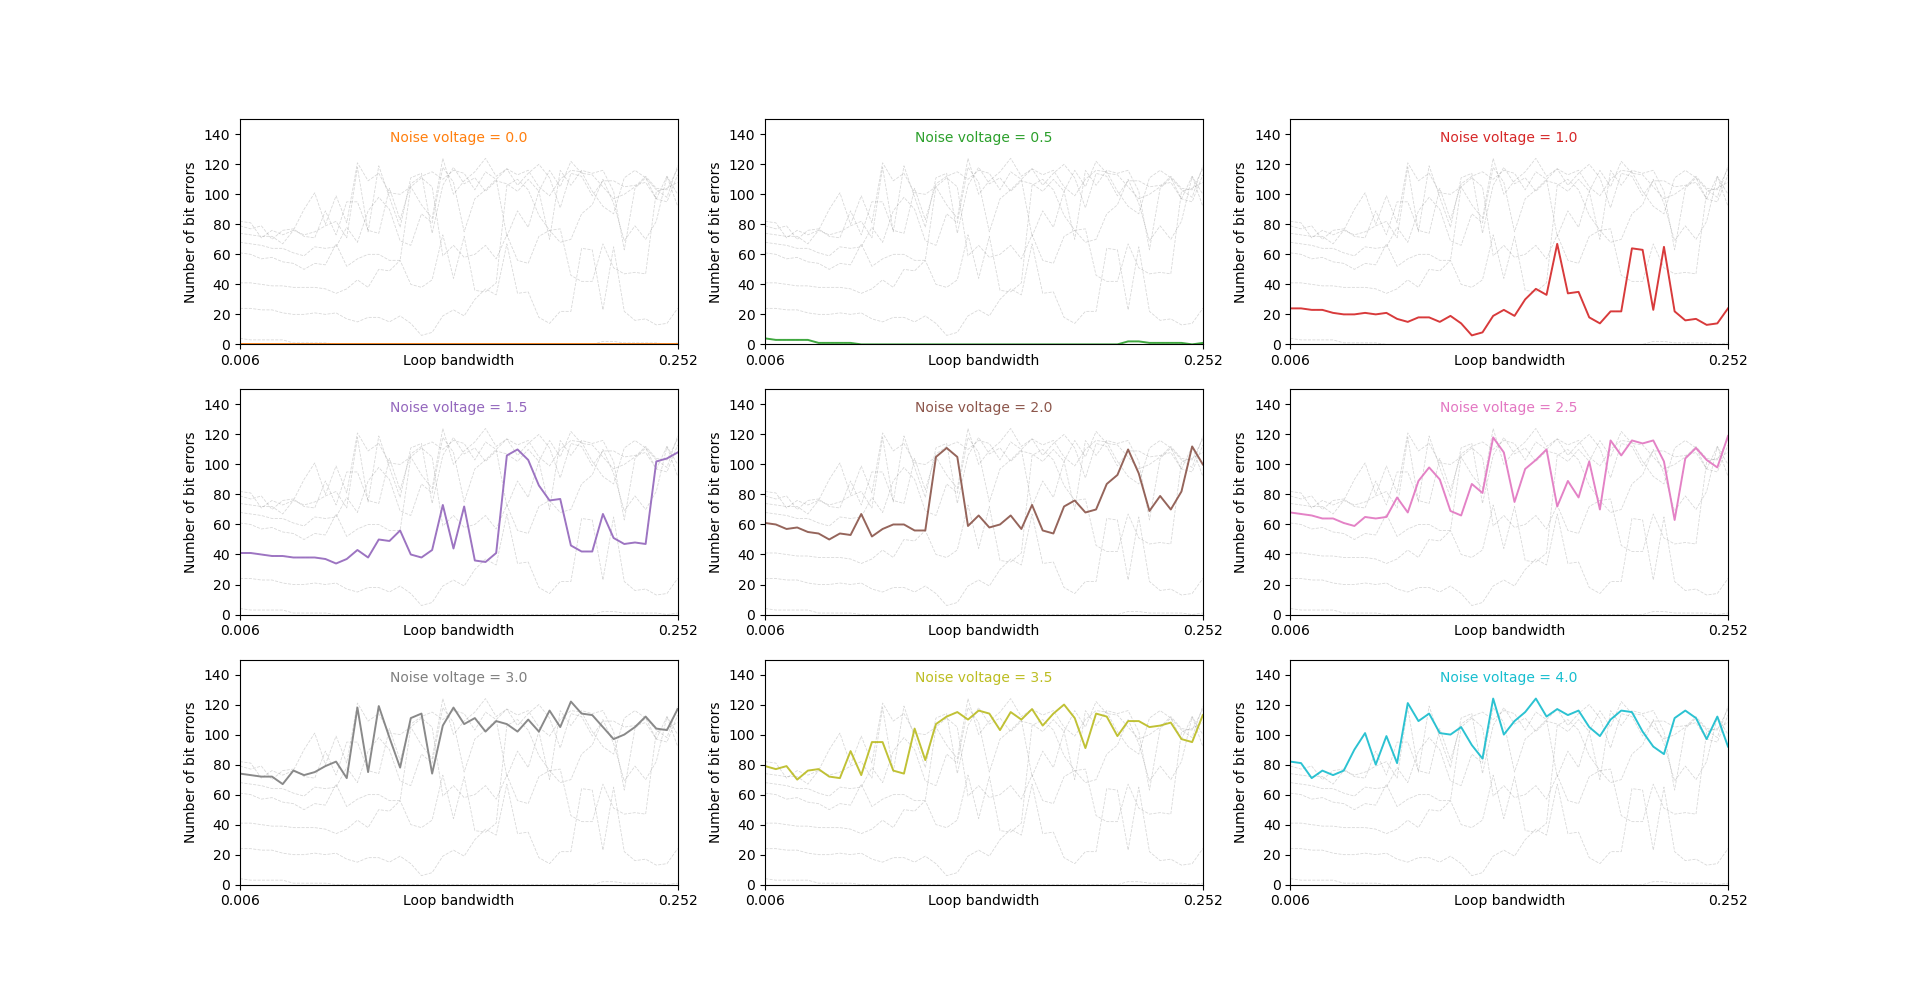
\includegraphics[width=1\linewidth]{img/analise/QPSK_9.png}
    \caption{Evolução do número de erros de bit para cada \textit{noise voltage}, em função da \textit{Loop Bandwidth}.}
    \label{fig:qpsk9}
\end{figure}

\noindent\fcolorbox{black}{white}{%
        \minipage[t]{\dimexpr\linewidth-2\fboxsep-2\fboxrule\relax}
            \textbf{Nota} $\rightarrow$ Os resultados e observações são bastante análogos à versão BPSK, pelo que se seguem as mesmas ilações. Salienta-se somente, para reforçar a ideia, que em média, a taxa de erro de \textit{bit} para cada patamar de ruído impõe precisamente a mesma evolução que no caso exposto anteriormente (vide \hyperref[fig:bpsk9]{Fig. E1} e \hyperref[tab:bpsk]{Tab. E1}). 
        \endminipage}